Sketch the feasible region.

\begin{solution}
    We begin by introducing variable transformations to convert the problem to a standard form. To do so, we define 
    $x_1' = -x_1 + 3$ and $x_2' = x_2 - 1$. We convert the program to a minimization problem by multiplying the 
    objective function by -1 to obtain $-z = x_1' - x_2' - 4$. We roll the constant term into the objective function
    and define the new objective function $\tilde{z} = x_1' - x_2'$ to obtain the system:

    \begin{mini*}
        {}{\tilde{z} = x_1' - x_2'}{}{}
        \addConstraint{x_1' + x_2'}{\le 2}
        \addConstraint{x_1', x_2'}{\ge 0}.
    \end{mini*}

    This system is plotted in Figure (\ref{fig:problem_5a}).

    \begin{figure}[h]
        \centering
        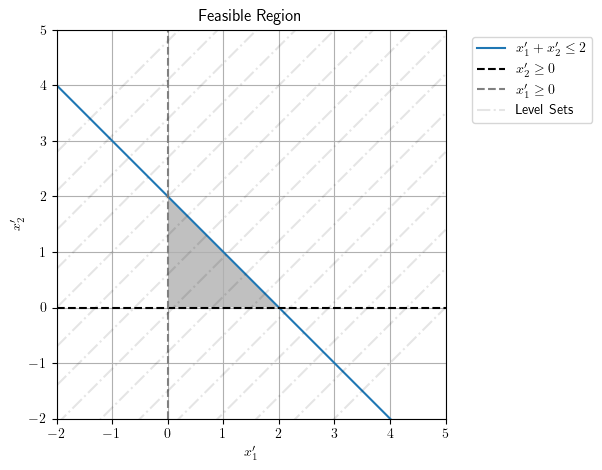
\includegraphics[width=0.6\textwidth]{problem_5a.png}
        \caption{Feasible region for 5(a)}
        \label{fig:problem_5a}
    \end{figure}
\end{solution}